% Options for packages loaded elsewhere
\PassOptionsToPackage{unicode}{hyperref}
\PassOptionsToPackage{hyphens}{url}
%
\documentclass[
]{book}
\usepackage{lmodern}
\usepackage{amsmath}
\usepackage{ifxetex,ifluatex}
\ifnum 0\ifxetex 1\fi\ifluatex 1\fi=0 % if pdftex
  \usepackage[T1]{fontenc}
  \usepackage[utf8]{inputenc}
  \usepackage{textcomp} % provide euro and other symbols
  \usepackage{amssymb}
\else % if luatex or xetex
  \usepackage{unicode-math}
  \defaultfontfeatures{Scale=MatchLowercase}
  \defaultfontfeatures[\rmfamily]{Ligatures=TeX,Scale=1}
\fi
% Use upquote if available, for straight quotes in verbatim environments
\IfFileExists{upquote.sty}{\usepackage{upquote}}{}
\IfFileExists{microtype.sty}{% use microtype if available
  \usepackage[]{microtype}
  \UseMicrotypeSet[protrusion]{basicmath} % disable protrusion for tt fonts
}{}
\makeatletter
\@ifundefined{KOMAClassName}{% if non-KOMA class
  \IfFileExists{parskip.sty}{%
    \usepackage{parskip}
  }{% else
    \setlength{\parindent}{0pt}
    \setlength{\parskip}{6pt plus 2pt minus 1pt}}
}{% if KOMA class
  \KOMAoptions{parskip=half}}
\makeatother
\usepackage{xcolor}
\IfFileExists{xurl.sty}{\usepackage{xurl}}{} % add URL line breaks if available
\IfFileExists{bookmark.sty}{\usepackage{bookmark}}{\usepackage{hyperref}}
\hypersetup{
  pdftitle={Tutorial Book: The Analysis of Distribution and Density Changes of Electric Vehicle Charging Points in London Boroughs},
  pdfauthor={Zeqiang Fang},
  hidelinks,
  pdfcreator={LaTeX via pandoc}}
\urlstyle{same} % disable monospaced font for URLs
\usepackage{color}
\usepackage{fancyvrb}
\newcommand{\VerbBar}{|}
\newcommand{\VERB}{\Verb[commandchars=\\\{\}]}
\DefineVerbatimEnvironment{Highlighting}{Verbatim}{commandchars=\\\{\}}
% Add ',fontsize=\small' for more characters per line
\usepackage{framed}
\definecolor{shadecolor}{RGB}{248,248,248}
\newenvironment{Shaded}{\begin{snugshade}}{\end{snugshade}}
\newcommand{\AlertTok}[1]{\textcolor[rgb]{0.94,0.16,0.16}{#1}}
\newcommand{\AnnotationTok}[1]{\textcolor[rgb]{0.56,0.35,0.01}{\textbf{\textit{#1}}}}
\newcommand{\AttributeTok}[1]{\textcolor[rgb]{0.77,0.63,0.00}{#1}}
\newcommand{\BaseNTok}[1]{\textcolor[rgb]{0.00,0.00,0.81}{#1}}
\newcommand{\BuiltInTok}[1]{#1}
\newcommand{\CharTok}[1]{\textcolor[rgb]{0.31,0.60,0.02}{#1}}
\newcommand{\CommentTok}[1]{\textcolor[rgb]{0.56,0.35,0.01}{\textit{#1}}}
\newcommand{\CommentVarTok}[1]{\textcolor[rgb]{0.56,0.35,0.01}{\textbf{\textit{#1}}}}
\newcommand{\ConstantTok}[1]{\textcolor[rgb]{0.00,0.00,0.00}{#1}}
\newcommand{\ControlFlowTok}[1]{\textcolor[rgb]{0.13,0.29,0.53}{\textbf{#1}}}
\newcommand{\DataTypeTok}[1]{\textcolor[rgb]{0.13,0.29,0.53}{#1}}
\newcommand{\DecValTok}[1]{\textcolor[rgb]{0.00,0.00,0.81}{#1}}
\newcommand{\DocumentationTok}[1]{\textcolor[rgb]{0.56,0.35,0.01}{\textbf{\textit{#1}}}}
\newcommand{\ErrorTok}[1]{\textcolor[rgb]{0.64,0.00,0.00}{\textbf{#1}}}
\newcommand{\ExtensionTok}[1]{#1}
\newcommand{\FloatTok}[1]{\textcolor[rgb]{0.00,0.00,0.81}{#1}}
\newcommand{\FunctionTok}[1]{\textcolor[rgb]{0.00,0.00,0.00}{#1}}
\newcommand{\ImportTok}[1]{#1}
\newcommand{\InformationTok}[1]{\textcolor[rgb]{0.56,0.35,0.01}{\textbf{\textit{#1}}}}
\newcommand{\KeywordTok}[1]{\textcolor[rgb]{0.13,0.29,0.53}{\textbf{#1}}}
\newcommand{\NormalTok}[1]{#1}
\newcommand{\OperatorTok}[1]{\textcolor[rgb]{0.81,0.36,0.00}{\textbf{#1}}}
\newcommand{\OtherTok}[1]{\textcolor[rgb]{0.56,0.35,0.01}{#1}}
\newcommand{\PreprocessorTok}[1]{\textcolor[rgb]{0.56,0.35,0.01}{\textit{#1}}}
\newcommand{\RegionMarkerTok}[1]{#1}
\newcommand{\SpecialCharTok}[1]{\textcolor[rgb]{0.00,0.00,0.00}{#1}}
\newcommand{\SpecialStringTok}[1]{\textcolor[rgb]{0.31,0.60,0.02}{#1}}
\newcommand{\StringTok}[1]{\textcolor[rgb]{0.31,0.60,0.02}{#1}}
\newcommand{\VariableTok}[1]{\textcolor[rgb]{0.00,0.00,0.00}{#1}}
\newcommand{\VerbatimStringTok}[1]{\textcolor[rgb]{0.31,0.60,0.02}{#1}}
\newcommand{\WarningTok}[1]{\textcolor[rgb]{0.56,0.35,0.01}{\textbf{\textit{#1}}}}
\usepackage{longtable,booktabs}
% Correct order of tables after \paragraph or \subparagraph
\usepackage{etoolbox}
\makeatletter
\patchcmd\longtable{\par}{\if@noskipsec\mbox{}\fi\par}{}{}
\makeatother
% Allow footnotes in longtable head/foot
\IfFileExists{footnotehyper.sty}{\usepackage{footnotehyper}}{\usepackage{footnote}}
\makesavenoteenv{longtable}
\usepackage{graphicx}
\makeatletter
\def\maxwidth{\ifdim\Gin@nat@width>\linewidth\linewidth\else\Gin@nat@width\fi}
\def\maxheight{\ifdim\Gin@nat@height>\textheight\textheight\else\Gin@nat@height\fi}
\makeatother
% Scale images if necessary, so that they will not overflow the page
% margins by default, and it is still possible to overwrite the defaults
% using explicit options in \includegraphics[width, height, ...]{}
\setkeys{Gin}{width=\maxwidth,height=\maxheight,keepaspectratio}
% Set default figure placement to htbp
\makeatletter
\def\fps@figure{htbp}
\makeatother
\setlength{\emergencystretch}{3em} % prevent overfull lines
\providecommand{\tightlist}{%
  \setlength{\itemsep}{0pt}\setlength{\parskip}{0pt}}
\setcounter{secnumdepth}{5}
\usepackage{booktabs}
\usepackage{amsthm}
\makeatletter
\def\thm@space@setup{%
  \thm@preskip=8pt plus 2pt minus 4pt
  \thm@postskip=\thm@preskip
}
\makeatother
\ifluatex
  \usepackage{selnolig}  % disable illegal ligatures
\fi
\usepackage[]{natbib}
\bibliographystyle{apalike}

\title{Tutorial Book: The Analysis of Distribution and Density Changes of Electric Vehicle Charging Points in London Boroughs}
\author{Zeqiang Fang}
\date{2021-01-15}

\begin{document}
\maketitle

{
\setcounter{tocdepth}{1}
\tableofcontents
}
\hypertarget{introduction-and-description-of-data}{%
\chapter{Introduction and Description of Data}\label{introduction-and-description-of-data}}

Electric vehicle (EV) infrastructure is of importance for sustainable urban development. ``UK e-charging market is recognised as one of the most advanced in Europe,'' said Martin Lucas. He is a partner of Watson Farley \& Williams LLP, an international law firm (2020). However, urban residents who purchase new energy vehicles have to face range anxiety, which has become a constraint on developing the EV market. EVs' sales are lower than expected because of the potential users' anxiety range (Bonges and Lusk, 2016).

In this report, the research question will be investigated and discussed --- How do the distribution and density of EV charge change in London between 2019 and 2020? The aim is to apply theories from GIS, especially the spatial analysis method, to explore the distribution and density in these two years. Firstly, the big data of charge points, from the UK government official website, is pre-processed and cleaned. One of the analysis methods is to apply spatial pattern analysis. It is based on the number of samples in two years. It compares their distribution and density to obtain the corresponding objective value. Besides, a reproducible analysis process is established using open source spatial analysis software RStudio, which applies the advanced spatial analysis methods in clean energy and explores spatial value content to contribute to urban sustainability.

\hypertarget{electric-vehicle-charge-point-dataset}{%
\section{Electric Vehicle Charge Point Dataset}\label{electric-vehicle-charge-point-dataset}}

The NCR, a database of charge points for electric vehicles in the UK, is available for individuals and business data developers without charge (GOV.UK, 2020). Following the UK government website's guidance, the National Chargepoint Registry (NCR) dataset was collected in CSV format.

You can access this dataset in this \href{https://www.gov.uk/guidance/find-and-use-data-on-public-electric-vehicle-chargepoints\#accessing-data-on-ncv}{link}. \textbf{OR}, you can also access this dataset in the \href{https://raw.githubusercontent.com/Hereislittlemushroom/CASA0005_Final_Assessment/main/Dataset/national-charge-point-registry.csv}{github}

\hypertarget{london-boroughs-geometric-dataset}{%
\section{London Boroughs Geometric Dataset}\label{london-boroughs-geometric-dataset}}

Spatial data is available on the London Datastore official website. The shape format file called Statistical GIS Boundary is the original geographic boundaries data, which is based on our spatial analysis (London Datastore, 2020). One of the variables called ``GSS\_CODE'' can be identified via ``sf,'' an R package, to present the London borough polygons in multiple types.

You should download this complete folder to read shape file! The link is \href{https://github.com/Hereislittlemushroom/CASA0005_Final_Assessment/tree/main/Dataset/statistical-gis-boundaries-london}{here}

\hypertarget{environment-preparation}{%
\chapter{Environment Preparation}\label{environment-preparation}}

\hypertarget{environment-recommendation}{%
\section{Environment Recommendation}\label{environment-recommendation}}

\begin{itemize}
\item
  System: MacOS 10.5 / 11.0 Windows 10
\item
  IDE: RStudio 1.3 (MacOS) R \textgreater= 3.6
\end{itemize}

\hypertarget{import-packages-for-spatial-analysis-and-map-making}{%
\section{Import packages for spatial analysis and map making}\label{import-packages-for-spatial-analysis-and-map-making}}

If there are errors take place, you can run \texttt{install.packages(\{missing\ package\ name\})} to install packages.

\begin{Shaded}
\begin{Highlighting}[]
\FunctionTok{library}\NormalTok{(tidyverse)}
\FunctionTok{library}\NormalTok{(data.table)}
\FunctionTok{library}\NormalTok{(sp)}
\FunctionTok{library}\NormalTok{(sf)}
\FunctionTok{library}\NormalTok{(table1)}
\FunctionTok{library}\NormalTok{(tm)}
\FunctionTok{library}\NormalTok{(spatstat)}
\FunctionTok{library}\NormalTok{(here)}
\FunctionTok{library}\NormalTok{(sp)}
\FunctionTok{library}\NormalTok{(rgeos)}
\CommentTok{\# library(maptools)}
\FunctionTok{library}\NormalTok{(tmap)}
\FunctionTok{library}\NormalTok{(sf)}
\FunctionTok{library}\NormalTok{(geojson)}
\FunctionTok{library}\NormalTok{(geojsonio)}
\FunctionTok{library}\NormalTok{(tmaptools)}
\FunctionTok{library}\NormalTok{(RColorBrewer)}
\FunctionTok{library}\NormalTok{(spdep) }
\FunctionTok{library}\NormalTok{(lubridate)}
\end{Highlighting}
\end{Shaded}

\hypertarget{data-pre-processing}{%
\chapter{Data Pre-processing}\label{data-pre-processing}}

\hypertarget{read-data-into-r}{%
\section{Read data into R}\label{read-data-into-r}}

The \textbf{National Chargepoint Register(NCR)} is a database of publicly-available chargepoints for electric vehicles in the UK established in 2011(,2021). you can access data in this \href{https://www.gov.uk/guidance/find-and-use-data-on-public-electric-vehicle-chargepoints\#accessing-data-on-ncv}{link}

Now, let's read original data in R

\begin{Shaded}
\begin{Highlighting}[]
\NormalTok{UK\_NCR}\OtherTok{=} \FunctionTok{read.csv}\NormalTok{(here}\SpecialCharTok{::}\FunctionTok{here}\NormalTok{(}\StringTok{"dataset"}\NormalTok{,}\StringTok{"national{-}charge{-}point{-}registry.csv"}\NormalTok{)) }
\CommentTok{\# This may take for a while, which depends on the speed of internet}

\CommentTok{\# you can have a overview of this dataset}
\FunctionTok{print}\NormalTok{(}\StringTok{"The number of rows is: "}\NormalTok{)}
\FunctionTok{nrow}\NormalTok{(UK\_NCR)}
\FunctionTok{print}\NormalTok{(}\StringTok{"The number of columns is: "}\NormalTok{)}
\FunctionTok{ncol}\NormalTok{(UK\_NCR)}
\FunctionTok{print}\NormalTok{(}\StringTok{"70 of all varriables are:"}\NormalTok{)}
\FunctionTok{head}\NormalTok{(}\FunctionTok{names}\NormalTok{(UK\_NCR),}\AttributeTok{n =} \DecValTok{70}\NormalTok{)}
\end{Highlighting}
\end{Shaded}

Tip: If you cannot successfully read this dataset, you can replace the above link with ``\url{https://raw.githubusercontent.com/Hereislittlemushroom/CASA0005_Final_Assessment/main/Dataset/national-charge-point-registry.csv}''

\hypertarget{data-selection}{%
\section{Data Selection}\label{data-selection}}

Select the charge points of london area in this UK csv file。
You can utilise \texttt{filter} function from \texttt{dplyr} package to choose the charge point data in london boroughs

\begin{Shaded}
\begin{Highlighting}[]
\NormalTok{London\_NCR }\OtherTok{=}\NormalTok{ UK\_NCR }\SpecialCharTok{\%\textgreater{}\%}
\NormalTok{  dplyr}\SpecialCharTok{::}\FunctionTok{filter}\NormalTok{(  }\SpecialCharTok{!}\FunctionTok{is.na}\NormalTok{(county),}
\NormalTok{                  county }\SpecialCharTok{==} \StringTok{"London"} \SpecialCharTok{|} 
\NormalTok{                  county }\SpecialCharTok{==} \StringTok{"Greater London "} \SpecialCharTok{|} 
\NormalTok{                  county }\SpecialCharTok{==} \StringTok{"London Borough of Camden"} \SpecialCharTok{|}
\NormalTok{                  county }\SpecialCharTok{==} \StringTok{"London Borough of Ealing"} \SpecialCharTok{|} 
\NormalTok{                  county }\SpecialCharTok{==} \StringTok{"London Borough of Greenwich"} \SpecialCharTok{|} 
\NormalTok{                  county }\SpecialCharTok{==} \StringTok{"London Borough of Hackney"} \SpecialCharTok{|} 
\NormalTok{                  county }\SpecialCharTok{==} \StringTok{"London Borough of Hammersmith and Fulham"} \SpecialCharTok{|} 
\NormalTok{                  county }\SpecialCharTok{==} \StringTok{"London Borough of Hounslow"} \SpecialCharTok{|} 
\NormalTok{                  county }\SpecialCharTok{==} \StringTok{"London Borough of Islington"} \SpecialCharTok{|} 
\NormalTok{                  county }\SpecialCharTok{==} \StringTok{"London Borough of Lambeth"} \SpecialCharTok{|} 
\NormalTok{                  county }\SpecialCharTok{==} \StringTok{"London Borough of Richmond upon Thames"} \SpecialCharTok{|} 
\NormalTok{                  county }\SpecialCharTok{==} \StringTok{"London Borough of Southwark"} \SpecialCharTok{|}
\NormalTok{                  county }\SpecialCharTok{==} \StringTok{"London Borough Of Southwark"} \SpecialCharTok{|}
\NormalTok{                  county }\SpecialCharTok{==} \StringTok{"London Borough of Waltham Forest"} \SpecialCharTok{|} 
\NormalTok{                  county }\SpecialCharTok{==} \StringTok{"London Borough of Wandsworth"}\NormalTok{)}
\end{Highlighting}
\end{Shaded}

Check if all values in \texttt{county} are attributed to ``London''

\begin{Shaded}
\begin{Highlighting}[]
\NormalTok{isLondon }\OtherTok{=}\NormalTok{ London\_NCR}\SpecialCharTok{$}\NormalTok{county }\SpecialCharTok{\%\textgreater{}\%}
  \FunctionTok{unique}\NormalTok{()}
\NormalTok{isLondon}
\end{Highlighting}
\end{Shaded}

In the next step, you can select the valuable attributes e.g.~latitude,longitude.

\begin{Shaded}
\begin{Highlighting}[]
\CommentTok{\# Tip: the index of data frame starts from 1}
\CommentTok{\# Select the variables by their index}
\NormalTok{London\_NCR }\OtherTok{=}\NormalTok{ London\_NCR }\SpecialCharTok{\%\textgreater{}\%}
  \FunctionTok{select}\NormalTok{(}\DecValTok{1}\NormalTok{,}\DecValTok{4}\NormalTok{,}\DecValTok{5}\NormalTok{,}\DecValTok{13}\NormalTok{,}\DecValTok{14}\NormalTok{,}\DecValTok{15}\NormalTok{,}\DecValTok{32}\NormalTok{,}\DecValTok{35}\NormalTok{,}\DecValTok{36}\NormalTok{,}\DecValTok{38}\NormalTok{,}\DecValTok{54}\NormalTok{)}

\CommentTok{\# Check the variables we have chosen and the number of rows \& cols}
\NormalTok{London\_NCR }\SpecialCharTok{\%\textgreater{}\%}
  \FunctionTok{names}\NormalTok{()}
\NormalTok{London\_NCR }\SpecialCharTok{\%\textgreater{}\%}
  \FunctionTok{nrow}\NormalTok{()}
\NormalTok{London\_NCR }\SpecialCharTok{\%\textgreater{}\%}
  \FunctionTok{ncol}\NormalTok{()}
\end{Highlighting}
\end{Shaded}

\hypertarget{data-cleaning}{%
\section{Data Cleaning}\label{data-cleaning}}

Map and visualisation play important roles in spatial analysis. To make a heat map for further research, you need to merge geographic information for each row in charge point dataset in the first place.

To begin with, import ``PostcodesioR''. This R package offer methods to match

\begin{Shaded}
\begin{Highlighting}[]
\CommentTok{\# install.packages("PostcodesioR")}
\FunctionTok{library}\NormalTok{(PostcodesioR)}
\end{Highlighting}
\end{Shaded}

Before applying ``for-loop'' method to fill values in \texttt{GSS\_CODE} by identifying \texttt{postcode}, you can add a new columns called \texttt{GSS\_CODE} in London\_NCR dataset.

\begin{Shaded}
\begin{Highlighting}[]
\CommentTok{\# Attentions: you can skip this chunk because the for{-}loop process can take for a quite long time (about 5 min).}
\CommentTok{\# It is not necessary to stick on it, just skip!}

\NormalTok{London\_NCR\_GSS\_Added }\OtherTok{=}\NormalTok{ London\_NCR }\SpecialCharTok{\%\textgreater{}\%}
  \FunctionTok{rowwise}\NormalTok{() }\SpecialCharTok{\%\textgreater{}\%}
  \FunctionTok{mutate}\NormalTok{(}\AttributeTok{GSS\_CODE =}\NormalTok{ postcode) }\SpecialCharTok{\%\textgreater{}\%}
  \CommentTok{\# Tip: it is essential to transform numerical data into one in character}
  \FunctionTok{mutate}\NormalTok{(}\AttributeTok{GSS\_CODE =} \FunctionTok{as.character}\NormalTok{(GSS\_CODE))}

\CommentTok{\# Pay attention to the for loop in dataframe, it starts from 1}

\NormalTok{i }\OtherTok{=} \DecValTok{1}
\ControlFlowTok{for}\NormalTok{ (val }\ControlFlowTok{in}\NormalTok{ London\_NCR\_GSS\_Added}\SpecialCharTok{$}\NormalTok{postcode) \{}
  \FunctionTok{try}\NormalTok{(\{ temp1 }\OtherTok{=}\NormalTok{ PostcodesioR}\SpecialCharTok{::}\FunctionTok{postcode\_lookup}\NormalTok{(val)}
        \ControlFlowTok{if}\NormalTok{(}\SpecialCharTok{!}\FunctionTok{is.null}\NormalTok{(temp))\{}
\NormalTok{          temp2 }\OtherTok{=}\NormalTok{ temp1}\SpecialCharTok{$}\NormalTok{admin\_district\_code[}\DecValTok{1}\NormalTok{]}
\NormalTok{          London\_NCR\_GSS\_Added}\SpecialCharTok{$}\NormalTok{GSS\_CODE[i] }\OtherTok{=}\NormalTok{ temp2}
\NormalTok{        \}}\ControlFlowTok{else}\NormalTok{\{}
\NormalTok{          London\_NCR\_GSS\_Added}\SpecialCharTok{$}\NormalTok{GSS\_CODE[i] }\OtherTok{=} \StringTok{""}
\NormalTok{        \}}
\NormalTok{        i }\OtherTok{=}\NormalTok{ i}\SpecialCharTok{+}\DecValTok{1}\NormalTok{ \}}
\NormalTok{      ,}\AttributeTok{silent =} \ConstantTok{TRUE}\NormalTok{)}
\NormalTok{\}}

\CommentTok{\# remove the rows whose value of \textasciigrave{}GSS\_CODE\textasciigrave{} is empty}
\CommentTok{\# There are limitations in this process because the rows missing \textasciigrave{}GSS\_CODE\textasciigrave{} cannot be included in the dataset, which can slightly affect the research results }

\NormalTok{London\_NCR\_GSS\_Added}\SpecialCharTok{$}\NormalTok{GSS\_CODE[London\_NCR\_GSS\_Added}\SpecialCharTok{$}\NormalTok{GSS\_CODE}\SpecialCharTok{==}\StringTok{""}\NormalTok{] }\OtherTok{=} \ConstantTok{NA}
\NormalTok{London\_NCR\_GSS\_Added }\OtherTok{=}\NormalTok{ London\_NCR\_GSS\_Added }\SpecialCharTok{\%\textgreater{}\%}
  \FunctionTok{filter}\NormalTok{(}\SpecialCharTok{!}\FunctionTok{is.na}\NormalTok{(GSS\_CODE))}
\end{Highlighting}
\end{Shaded}

Finally, it is of importance to export our prepossessed data into csv file! Now we get the London\_NCR\_GSS\_Added.csv in our ``/Dataset'' path.

\begin{Shaded}
\begin{Highlighting}[]
\CommentTok{\# export London\_NCR\_GSS\_Added data frame into .CSV format}
\FunctionTok{library}\NormalTok{(here)}
\FunctionTok{write.csv}\NormalTok{(London\_NCR\_GSS\_Added, here}\SpecialCharTok{::}\FunctionTok{here}\NormalTok{(}\StringTok{"Dataset"}\NormalTok{,}\StringTok{"London\_NCR\_GSS\_Added.csv"}\NormalTok{), }\AttributeTok{row.names =} \ConstantTok{FALSE}\NormalTok{, }\AttributeTok{col.names =} \ConstantTok{TRUE}\NormalTok{)}
\CommentTok{\# \textasciigrave{}col.names = TRUE\textasciigrave{} is important to be writen down}
\end{Highlighting}
\end{Shaded}

Also, you can access this prepocessed dataset in github link:
\url{https://raw.githubusercontent.com/Hereislittlemushroom/CASA0005_Final_Assessment/main/Dataset/London_NCR_GSS_Added.csv}

\hypertarget{basic-settings}{%
\chapter{Basic Settings}\label{basic-settings}}

In this section, you will set the work path, import R packages, download the shape file \& its folder and read datasets in RStudio.

\hypertarget{set-the-path-of-your-project.}{%
\section{Set the path of your project.}\label{set-the-path-of-your-project.}}

Before you do the research, you should set the default path. The path below is mine, you should set your \textbf{own work path}

\begin{Shaded}
\begin{Highlighting}[]
\FunctionTok{setwd}\NormalTok{(}\StringTok{"/Users/fangzeqiang/Github/tutorial\_bookdown/"}\NormalTok{)}
\end{Highlighting}
\end{Shaded}

\hypertarget{import-the-shape-file}{%
\section{Import the shape file}\label{import-the-shape-file}}

What you should keep in mind is that this shape file should be run in the complete ESRI dir because there are some dependent files that the shape file might use.

\begin{Shaded}
\begin{Highlighting}[]
\CommentTok{\# you can download these files from github to your local work path that you set above}
\CommentTok{\# github link: https://github.com/Hereislittlemushroom/CASA0005\_Final\_Assessment/tree/main/Dataset/statistical{-}gis{-}boundaries{-}london}

\NormalTok{London\_Borough }\OtherTok{=} \FunctionTok{st\_read}\NormalTok{(}\StringTok{"dataset/statistical{-}gis{-}boundaries{-}london/ESRI/London\_Borough\_Excluding\_MHW.shp"}\NormalTok{)}
\end{Highlighting}
\end{Shaded}

\begin{verbatim}
## Reading layer `London_Borough_Excluding_MHW' from data source `/Users/fangzeqiang/Github/tutorial_bookdown/dataset/statistical-gis-boundaries-london/ESRI/London_Borough_Excluding_MHW.shp' using driver `ESRI Shapefile'
## Simple feature collection with 33 features and 7 fields
## geometry type:  MULTIPOLYGON
## dimension:      XY
## bbox:           xmin: 503568.2 ymin: 155850.8 xmax: 561957.5 ymax: 200933.9
## CRS:            27700
\end{verbatim}

\begin{Shaded}
\begin{Highlighting}[]
\CommentTok{\# plot the map}
\FunctionTok{plot}\NormalTok{(}\FunctionTok{st\_geometry}\NormalTok{(London\_Borough))}
\end{Highlighting}
\end{Shaded}

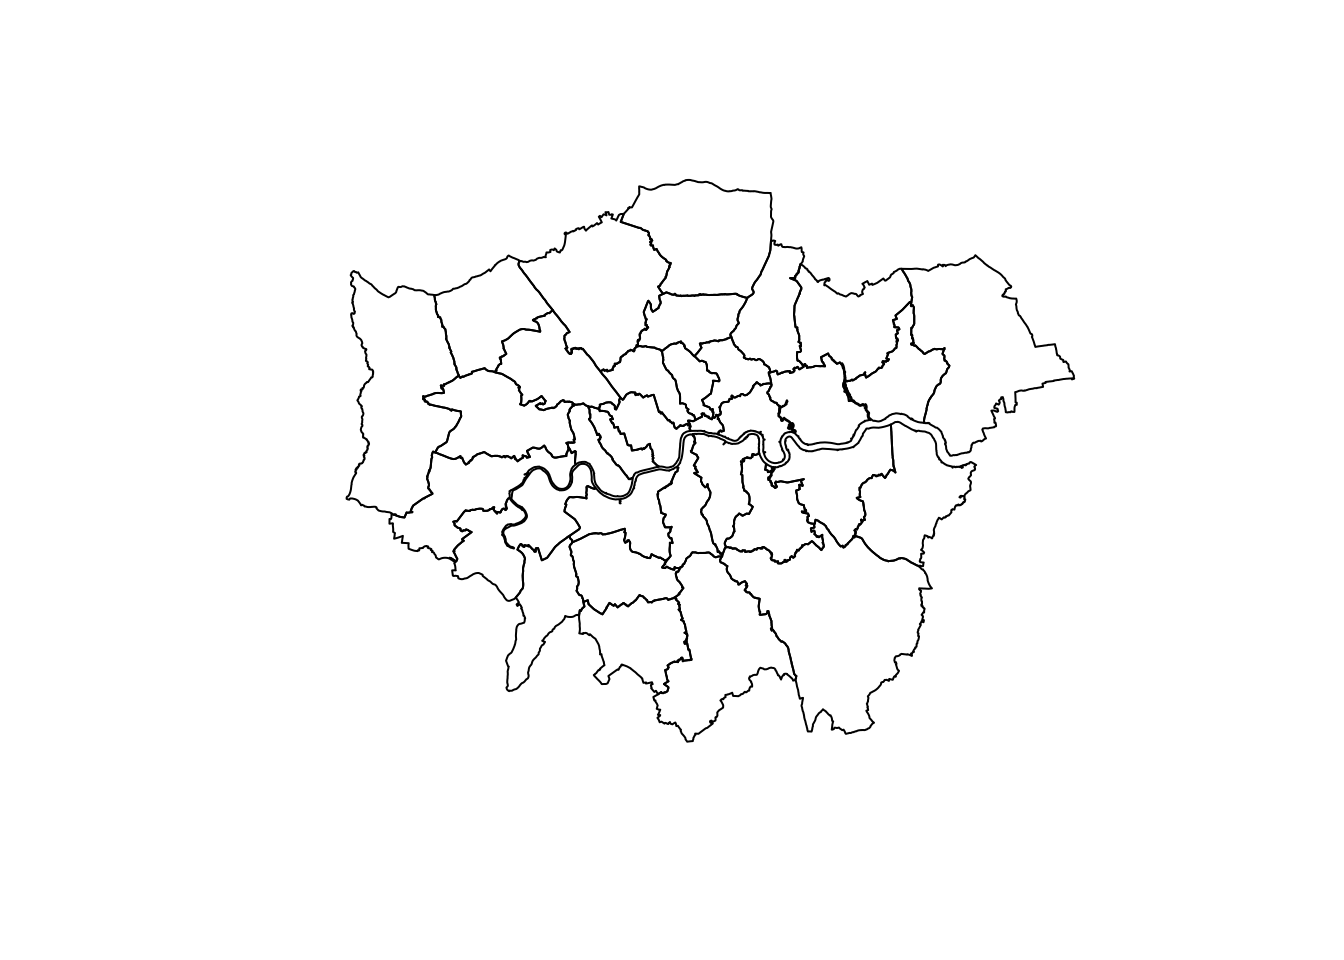
\includegraphics{bookdown-demo_files/figure-latex/unnamed-chunk-10-1.pdf}

\hypertarget{import-the-processed-london-national-chargepoint-register-ncr-dataset}{%
\section{Import the processed London national chargepoint register (NCR) dataset}\label{import-the-processed-london-national-chargepoint-register-ncr-dataset}}

The reason why choosing \texttt{fread} to read is because the read method is faster than the traditional ones. You can read .CSV file by \texttt{df\ =\ fread("Dataset/London\_NCR\_GSS\_Added.csv")}. However, in the following codes, I recommend that you read the pre-processed dataset from my github link.

\begin{Shaded}
\begin{Highlighting}[]
\CommentTok{\# df = fread("Dataset/London\_NCR\_GSS\_Added.csv")}
\CommentTok{\# df = fread(here::here("dataset","London\_NCR\_GSS\_Added.csv"))}
\CommentTok{\# df = fread("http://zeqiang.fun/\_book/dataset/London\_NCR\_GSS\_Added.csv")}
\NormalTok{ df }\OtherTok{=} \FunctionTok{fread}\NormalTok{(}\StringTok{"http://raw.githubusercontent.com/Hereislittlemushroom/CASA0005\_Final\_Assessment/main/Dataset/London\_NCR\_GSS\_Added.csv"}\NormalTok{)}
\end{Highlighting}
\end{Shaded}

\hypertarget{the-distribution-analysis-of-samples}{%
\chapter{The Distribution analysis of samples}\label{the-distribution-analysis-of-samples}}

You can generate a formal table to overview the distribution of samples. In order to compare samples between 2019 and 2020, you can obtain year from ``dataCreated'' which is timestamp format. Then you can create two columns in table (2019 \& 2020).

\begin{Shaded}
\begin{Highlighting}[]
\CommentTok{\#3.1 select the years}
\NormalTok{df}\SpecialCharTok{$}\NormalTok{year }\OtherTok{=} \FunctionTok{year}\NormalTok{(df}\SpecialCharTok{$}\NormalTok{dateCreated)}
\FunctionTok{table}\NormalTok{(df}\SpecialCharTok{$}\NormalTok{year)}
\end{Highlighting}
\end{Shaded}

\begin{verbatim}
## 
## 2017 2018 2019 2020 2021 
##    1    4  696  362    3
\end{verbatim}

\begin{Shaded}
\begin{Highlighting}[]
\CommentTok{\#select 2019 \& 2020 }
\NormalTok{df }\OtherTok{=}\NormalTok{ df[year}\SpecialCharTok{==}\DecValTok{2019}\SpecialCharTok{|}\NormalTok{year}\SpecialCharTok{==}\DecValTok{2020}\NormalTok{,]}
\FunctionTok{table}\NormalTok{(df}\SpecialCharTok{$}\NormalTok{year)}
\end{Highlighting}
\end{Shaded}

\begin{verbatim}
## 
## 2019 2020 
##  696  362
\end{verbatim}

\begin{Shaded}
\begin{Highlighting}[]
\CommentTok{\#3.2 show the table of the distribution of two years samples}
\FunctionTok{table1}\NormalTok{(}\SpecialCharTok{\textasciitilde{}}\NormalTok{county}\SpecialCharTok{|}\FunctionTok{factor}\NormalTok{(year),}\AttributeTok{data=}\NormalTok{df)}
\end{Highlighting}
\end{Shaded}

\begin{verbatim}
## [1] "<table class=\"Rtable1\">\n<thead>\n<tr>\n<th class='rowlabel firstrow lastrow'></th>\n<th class='firstrow lastrow'><span class='stratlabel'>2019<br><span class='stratn'>(N=696)</span></span></th>\n<th class='firstrow lastrow'><span class='stratlabel'>2020<br><span class='stratn'>(N=362)</span></span></th>\n<th class='firstrow lastrow'><span class='stratlabel'>Overall<br><span class='stratn'>(N=1058)</span></span></th>\n</tr>\n</thead>\n<tbody>\n<tr>\n<td class='rowlabel firstrow'><span class='varlabel'>county</span></td>\n<td class='firstrow'></td>\n<td class='firstrow'></td>\n<td class='firstrow'></td>\n</tr>\n<tr>\n<td class='rowlabel'>London</td>\n<td>150 (21.6%)</td>\n<td>150 (41.4%)</td>\n<td>300 (28.4%)</td>\n</tr>\n<tr>\n<td class='rowlabel'>London Borough of Camden</td>\n<td>87 (12.5%)</td>\n<td>179 (49.4%)</td>\n<td>266 (25.1%)</td>\n</tr>\n<tr>\n<td class='rowlabel'>London Borough of Ealing</td>\n<td>65 (9.3%)</td>\n<td>1 (0.3%)</td>\n<td>66 (6.2%)</td>\n</tr>\n<tr>\n<td class='rowlabel'>London Borough of Greenwich</td>\n<td>2 (0.3%)</td>\n<td>0 (0%)</td>\n<td>2 (0.2%)</td>\n</tr>\n<tr>\n<td class='rowlabel'>London Borough of Hackney</td>\n<td>62 (8.9%)</td>\n<td>0 (0%)</td>\n<td>62 (5.9%)</td>\n</tr>\n<tr>\n<td class='rowlabel'>London Borough of Hammersmith and Fulham</td>\n<td>2 (0.3%)</td>\n<td>3 (0.8%)</td>\n<td>5 (0.5%)</td>\n</tr>\n<tr>\n<td class='rowlabel'>London Borough of Hounslow</td>\n<td>78 (11.2%)</td>\n<td>0 (0%)</td>\n<td>78 (7.4%)</td>\n</tr>\n<tr>\n<td class='rowlabel'>London Borough of Islington</td>\n<td>3 (0.4%)</td>\n<td>15 (4.1%)</td>\n<td>18 (1.7%)</td>\n</tr>\n<tr>\n<td class='rowlabel'>London Borough of Lambeth</td>\n<td>118 (17.0%)</td>\n<td>2 (0.6%)</td>\n<td>120 (11.3%)</td>\n</tr>\n<tr>\n<td class='rowlabel'>London Borough of Richmond upon Thames</td>\n<td>8 (1.1%)</td>\n<td>9 (2.5%)</td>\n<td>17 (1.6%)</td>\n</tr>\n<tr>\n<td class='rowlabel'>London Borough of Southwark</td>\n<td>1 (0.1%)</td>\n<td>0 (0%)</td>\n<td>1 (0.1%)</td>\n</tr>\n<tr>\n<td class='rowlabel'>London Borough Of Southwark</td>\n<td>57 (8.2%)</td>\n<td>0 (0%)</td>\n<td>57 (5.4%)</td>\n</tr>\n<tr>\n<td class='rowlabel'>London Borough of Waltham Forest</td>\n<td>60 (8.6%)</td>\n<td>2 (0.6%)</td>\n<td>62 (5.9%)</td>\n</tr>\n<tr>\n<td class='rowlabel lastrow'>London Borough of Wandsworth</td>\n<td class='lastrow'>3 (0.4%)</td>\n<td class='lastrow'>1 (0.3%)</td>\n<td class='lastrow'>4 (0.4%)</td>\n</tr>\n</tbody>\n</table>\n"
\end{verbatim}

\begin{Shaded}
\begin{Highlighting}[]
\CommentTok{\# head(df)}
\end{Highlighting}
\end{Shaded}

\hypertarget{visualisation-and-comparison-of-the-density-of-london-ev-charge-point-between-two-years}{%
\chapter{Visualisation and comparison of the density of London EV charge point between two years}\label{visualisation-and-comparison-of-the-density-of-london-ev-charge-point-between-two-years}}

\hypertarget{data-cleaning-for-mapping}{%
\section{Data cleaning for mapping}\label{data-cleaning-for-mapping}}

You should split the NCR dataset to two dataset of two years, and merged these two processed dataset with geometric data respectively. Then we calculate the density for two years. Finally we can visualise and map the density

\begin{Shaded}
\begin{Highlighting}[]
\CommentTok{\#5.1 process the data to divide them by years(2019 \& 2020)}
\NormalTok{df1}\OtherTok{\textless{}{-}}\FunctionTok{subset}\NormalTok{(df,year}\SpecialCharTok{==}\DecValTok{2019}\NormalTok{) }\CommentTok{\#2019 year}
\NormalTok{df2}\OtherTok{\textless{}{-}}\FunctionTok{subset}\NormalTok{(df,year}\SpecialCharTok{==}\DecValTok{2020}\NormalTok{) }\CommentTok{\#2020 year}

\CommentTok{\# EV charge points created in 2019}
\CommentTok{\# sdf1\textless{}{-}merge(London\_Borough,df1,by="GSS\_CODE")}
\NormalTok{sdf1}\OtherTok{\textless{}{-}}\FunctionTok{merge}\NormalTok{(London\_Borough,df1,}\AttributeTok{by=}\StringTok{"GSS\_CODE"}\NormalTok{,}\AttributeTok{all =} \ConstantTok{TRUE}\NormalTok{)}
\NormalTok{sdf1}\OtherTok{\textless{}{-}}\NormalTok{sdf1[,}\FunctionTok{c}\NormalTok{(}\StringTok{"GSS\_CODE"}\NormalTok{,}\StringTok{"geometry"}\NormalTok{,}\StringTok{"longitude"}\NormalTok{,}\StringTok{"latitude"}\NormalTok{)]}

\CommentTok{\# EV charge points created in 2020}
\CommentTok{\# sdf2\textless{}{-}merge(London\_Borough,df2,by="GSS\_CODE")}
\NormalTok{sdf2}\OtherTok{\textless{}{-}}\FunctionTok{merge}\NormalTok{(London\_Borough,df2,}\AttributeTok{by=}\StringTok{"GSS\_CODE"}\NormalTok{,}\AttributeTok{all =} \ConstantTok{TRUE}\NormalTok{)}
\NormalTok{sdf2}\OtherTok{\textless{}{-}}\NormalTok{sdf2[,}\FunctionTok{c}\NormalTok{(}\StringTok{"GSS\_CODE"}\NormalTok{,}\StringTok{"geometry"}\NormalTok{,}\StringTok{"longitude"}\NormalTok{,}\StringTok{"latitude"}\NormalTok{)]}
\end{Highlighting}
\end{Shaded}

\hypertarget{the-density-of-data-in-2019}{%
\section{The density of data in 2019}\label{the-density-of-data-in-2019}}

First, you should calculate the density and transform the unit of area from m\^{}2 o km\^{}2. Then, select the necessary columns and add frequency of samples grouped by \texttt{GSS\_CODE}. In other words, you get the numeric and spatial data of EV charge point for each borough of London.

\begin{Shaded}
\begin{Highlighting}[]
\CommentTok{\# Data preparation}
\NormalTok{nsdf1 }\OtherTok{=}\NormalTok{ sdf1}\SpecialCharTok{\%\textgreater{}\%}
  \FunctionTok{add\_count}\NormalTok{(GSS\_CODE)}\SpecialCharTok{\%\textgreater{}\%}
  \FunctionTok{mutate}\NormalTok{(}\AttributeTok{area=}\FunctionTok{st\_area}\NormalTok{(.))}\SpecialCharTok{\%\textgreater{}\%}
  \CommentTok{\# Use dplyr::mutate to calculate the density of the charge point for each borough}
  \FunctionTok{mutate}\NormalTok{(}\AttributeTok{density=}\NormalTok{n}\SpecialCharTok{*}\DecValTok{1000}\SpecialCharTok{*}\DecValTok{1000}\SpecialCharTok{/}\NormalTok{area)}
  \CommentTok{\# because the st\_area default unit is square metre}

\CommentTok{\# select the following variables{-}{-}{-}"density","GSS\_CODE","n"(the count of GSS\_CODE)}
\NormalTok{nsdf1 }\OtherTok{=}\NormalTok{ dplyr}\SpecialCharTok{::}\FunctionTok{select}\NormalTok{(nsdf1,density,GSS\_CODE, n)}

\NormalTok{nsdf1 }\OtherTok{=}\NormalTok{ nsdf1}\SpecialCharTok{\%\textgreater{}\%}                    
  \FunctionTok{group\_by}\NormalTok{(GSS\_CODE)}\SpecialCharTok{\%\textgreater{}\%}         
  \FunctionTok{summarise}\NormalTok{(}\AttributeTok{density =}\FunctionTok{first}\NormalTok{(density),}\AttributeTok{GSS\_CODE=}\FunctionTok{first}\NormalTok{(GSS\_CODE))}
\end{Highlighting}
\end{Shaded}

\begin{verbatim}
## `summarise()` ungrouping output (override with `.groups` argument)
\end{verbatim}

Now you can generate map after setting some variables in \texttt{tmap\_mode}, \texttt{tm\_compass} and \texttt{tm\_polygons}.

\begin{Shaded}
\begin{Highlighting}[]
\FunctionTok{tmap\_mode}\NormalTok{(}\StringTok{"plot"}\NormalTok{)}
\end{Highlighting}
\end{Shaded}

\begin{verbatim}
## tmap mode set to plotting
\end{verbatim}

\begin{Shaded}
\begin{Highlighting}[]
\CommentTok{\# plot the figure: The distribution of the density of the London charge points in 2019}
\FunctionTok{tm\_shape}\NormalTok{( nsdf1) }\SpecialCharTok{+}
  \FunctionTok{tm\_compass}\NormalTok{( }\AttributeTok{north =} \DecValTok{0}\NormalTok{,}
              \AttributeTok{type =} \StringTok{"4star"}\NormalTok{,}
              \AttributeTok{text.size =} \FloatTok{0.8}\NormalTok{,}
              \AttributeTok{size =} \FloatTok{2.5}\NormalTok{,}
              \AttributeTok{show.labels =} \DecValTok{1}\NormalTok{,}
              \AttributeTok{cardinal.directions =} \FunctionTok{c}\NormalTok{(}\StringTok{"N"}\NormalTok{, }\StringTok{"E"}\NormalTok{, }\StringTok{"S"}\NormalTok{, }\StringTok{"W"}\NormalTok{),}
              \AttributeTok{lwd =} \DecValTok{1}\NormalTok{,}
              \AttributeTok{position =} \FunctionTok{c}\NormalTok{(}\StringTok{"left"}\NormalTok{,}\StringTok{"top"}\NormalTok{),}
              \AttributeTok{bg.color =} \ConstantTok{NA}\NormalTok{,}
              \AttributeTok{bg.alpha =} \ConstantTok{NA}\NormalTok{,}
              \AttributeTok{just =} \ConstantTok{NA}\NormalTok{,}
              \AttributeTok{fontsize =} \FloatTok{1.5}\NormalTok{) }\SpecialCharTok{+}
  \FunctionTok{tm\_polygons}\NormalTok{(}\StringTok{"density"}\NormalTok{,}
              \AttributeTok{style=}\StringTok{"jenks"}\NormalTok{,}
              \AttributeTok{palette=}\StringTok{"RdPu"}\NormalTok{,}
              \AttributeTok{midpoint=}\ConstantTok{NA}\NormalTok{,}
              \AttributeTok{popup.vars=}\FunctionTok{c}\NormalTok{(}\StringTok{"GSS\_CODE"}\NormalTok{, }\StringTok{"density"}\NormalTok{),}
              \AttributeTok{title=}\StringTok{"Density per square kilometre (2019)"}
\NormalTok{              )}
\end{Highlighting}
\end{Shaded}

\begin{verbatim}
## Warning: The argument fontsize of tm_compass is deprecated. It has been renamed
## to text.size
\end{verbatim}

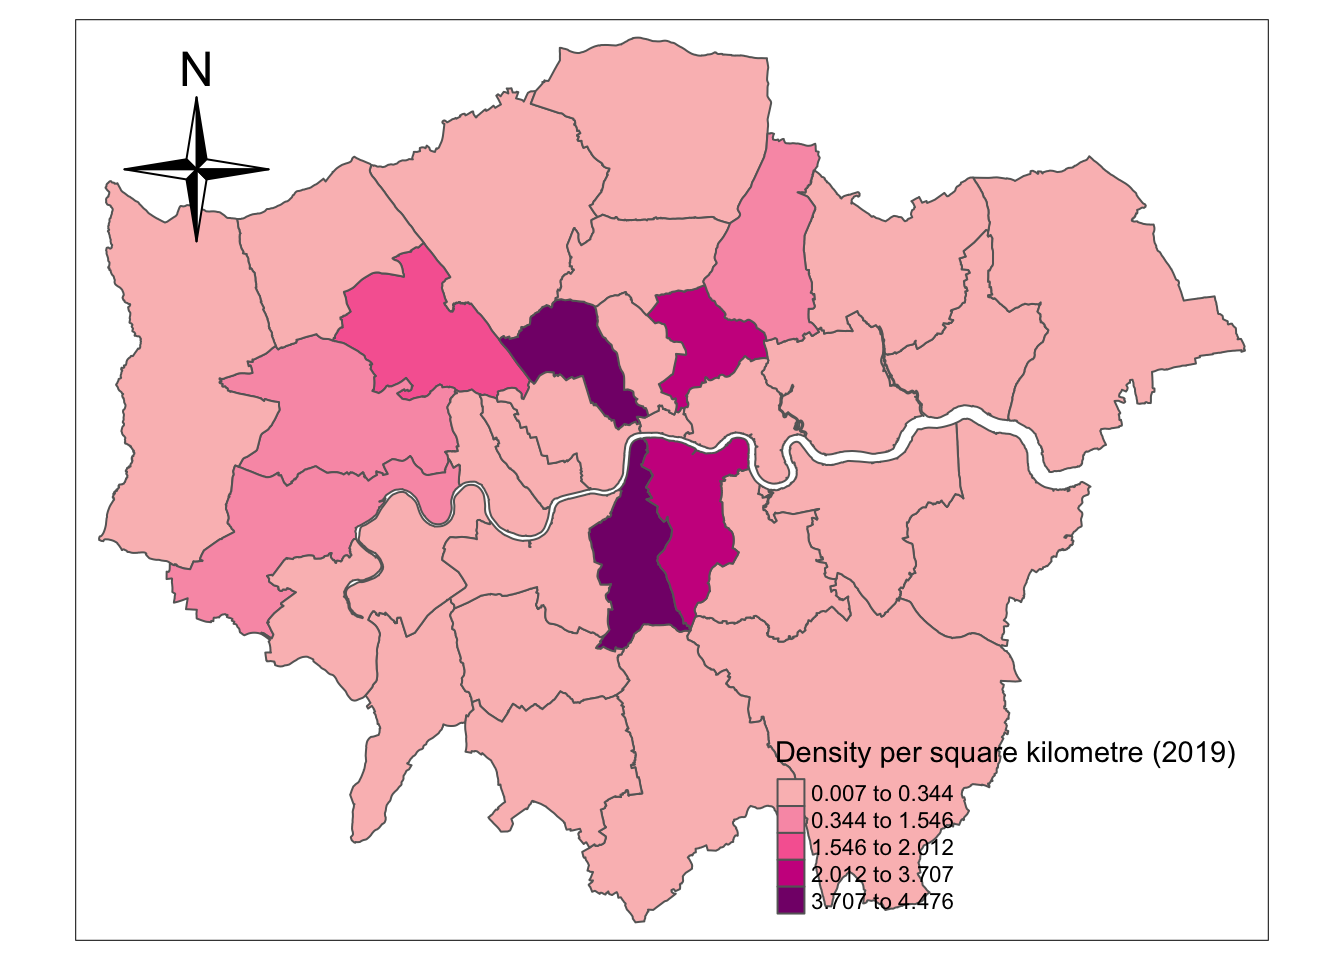
\includegraphics{bookdown-demo_files/figure-latex/unnamed-chunk-15-1.pdf}

\hypertarget{the-density-of-data-in-2020}{%
\section{The density of data in 2020}\label{the-density-of-data-in-2020}}

Then you should conduct the similar process as the 4.2 section to draw the density of EV charge point data in 2020.

\begin{Shaded}
\begin{Highlighting}[]
\NormalTok{nsdf2 }\OtherTok{=}\NormalTok{ sdf2}\SpecialCharTok{\%\textgreater{}\%}
  \FunctionTok{add\_count}\NormalTok{(GSS\_CODE)}\SpecialCharTok{\%\textgreater{}\%}
  \FunctionTok{mutate}\NormalTok{(}\AttributeTok{area=}\FunctionTok{st\_area}\NormalTok{(.))}\SpecialCharTok{\%\textgreater{}\%}
  \FunctionTok{mutate}\NormalTok{(units}\SpecialCharTok{::}\FunctionTok{set\_units}\NormalTok{(area,km}\SpecialCharTok{\^{}}\DecValTok{2}\NormalTok{))}\SpecialCharTok{\%\textgreater{}\%}
  \FunctionTok{mutate}\NormalTok{(}\AttributeTok{density=}\NormalTok{n}\SpecialCharTok{*}\DecValTok{1000}\SpecialCharTok{*}\DecValTok{1000}\SpecialCharTok{/}\NormalTok{area)}

\NormalTok{nsdf2 }\OtherTok{=}\NormalTok{ dplyr}\SpecialCharTok{::}\FunctionTok{select}\NormalTok{(nsdf2,density,GSS\_CODE, n)}

\NormalTok{nsdf2 }\OtherTok{=}\NormalTok{ nsdf2}\SpecialCharTok{\%\textgreater{}\%}                    
  \FunctionTok{group\_by}\NormalTok{(GSS\_CODE)}\SpecialCharTok{\%\textgreater{}\%}         
  \FunctionTok{summarise}\NormalTok{(}\AttributeTok{density =}\FunctionTok{first}\NormalTok{(density),}\AttributeTok{GSS\_CODE=}\FunctionTok{first}\NormalTok{(GSS\_CODE))}
\end{Highlighting}
\end{Shaded}

\begin{verbatim}
## `summarise()` ungrouping output (override with `.groups` argument)
\end{verbatim}

\begin{Shaded}
\begin{Highlighting}[]
\FunctionTok{tmap\_mode}\NormalTok{(}\StringTok{"plot"}\NormalTok{)}
\end{Highlighting}
\end{Shaded}

\begin{verbatim}
## tmap mode set to plotting
\end{verbatim}

\begin{Shaded}
\begin{Highlighting}[]
\FunctionTok{tm\_shape}\NormalTok{( nsdf2) }\SpecialCharTok{+}
  \FunctionTok{tm\_compass}\NormalTok{( }\AttributeTok{north =} \DecValTok{0}\NormalTok{,}
              \AttributeTok{type =} \StringTok{"4star"}\NormalTok{,}
              \AttributeTok{text.size =} \FloatTok{0.8}\NormalTok{,}
              \AttributeTok{size =} \FloatTok{2.5}\NormalTok{,}
              \AttributeTok{show.labels =} \DecValTok{1}\NormalTok{,}
              \AttributeTok{cardinal.directions =} \FunctionTok{c}\NormalTok{(}\StringTok{"N"}\NormalTok{, }\StringTok{"E"}\NormalTok{, }\StringTok{"S"}\NormalTok{, }\StringTok{"W"}\NormalTok{),}
              \AttributeTok{lwd =} \DecValTok{1}\NormalTok{,}
              \AttributeTok{position =} \FunctionTok{c}\NormalTok{(}\StringTok{"left"}\NormalTok{,}\StringTok{"top"}\NormalTok{),}
              \AttributeTok{bg.color =} \ConstantTok{NA}\NormalTok{,}
              \AttributeTok{bg.alpha =} \ConstantTok{NA}\NormalTok{,}
              \AttributeTok{just =} \ConstantTok{NA}\NormalTok{,}
              \AttributeTok{fontsize =} \FloatTok{1.5}\NormalTok{) }\SpecialCharTok{+}
  \FunctionTok{tm\_polygons}\NormalTok{(}\StringTok{"density"}\NormalTok{,}
              \AttributeTok{style=}\StringTok{"jenks"}\NormalTok{,}
              \AttributeTok{palette=}\StringTok{"PuOr"}\NormalTok{,}
              \AttributeTok{midpoint=}\ConstantTok{NA}\NormalTok{,}
              \AttributeTok{popup.vars=}\FunctionTok{c}\NormalTok{(}\StringTok{"GSS\_CODE"}\NormalTok{, }\StringTok{"density"}\NormalTok{),}
              \AttributeTok{title=}\StringTok{"Density per square kilometre (2020)"}\NormalTok{)}
\end{Highlighting}
\end{Shaded}

\begin{verbatim}
## Warning: The argument fontsize of tm_compass is deprecated. It has been renamed
## to text.size
\end{verbatim}

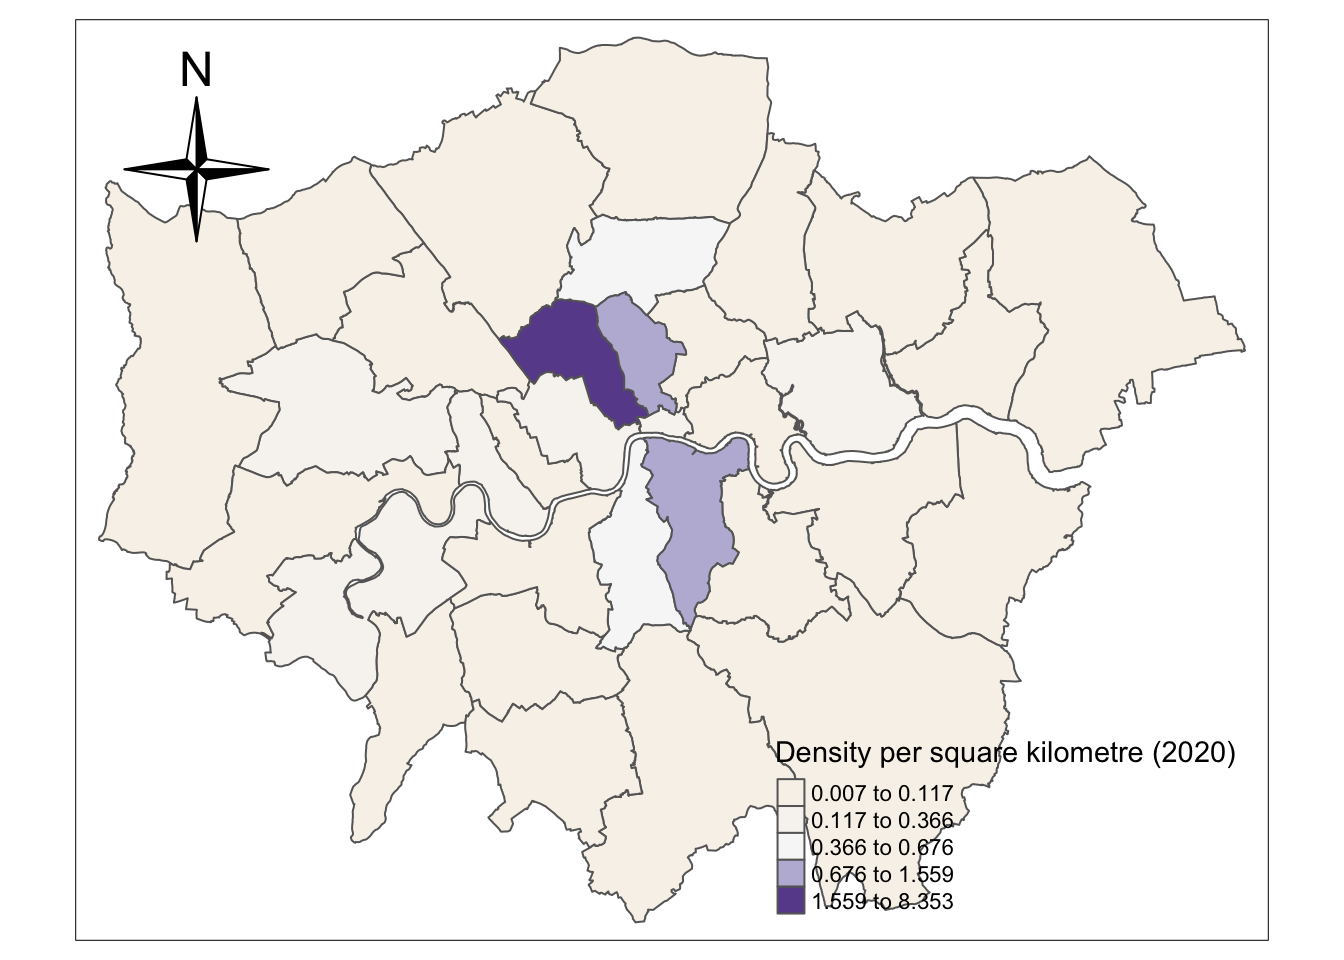
\includegraphics{bookdown-demo_files/figure-latex/unnamed-chunk-16-1.pdf}

\hypertarget{analysing-spatial-autocorrelation-with-morans-i}{%
\chapter{Analysing Spatial Autocorrelation with Moran's I}\label{analysing-spatial-autocorrelation-with-morans-i}}

Since the sample in 2019 \& 2020 is too small to run a good result, you can analysis the autocorrelation based on the samples which contain these two years.

\hypertarget{generate-the-data-for-analysis}{%
\section{Generate the data for analysis}\label{generate-the-data-for-analysis}}

This process is similar to the 4.2 and 4.3 data preparation.

\begin{Shaded}
\begin{Highlighting}[]
\NormalTok{sdf }\OtherTok{=} \FunctionTok{merge}\NormalTok{(London\_Borough,df,}\AttributeTok{by=}\StringTok{"GSS\_CODE"}\NormalTok{,}\AttributeTok{all =} \ConstantTok{TRUE}\NormalTok{)}
\NormalTok{sdf }\OtherTok{=}\NormalTok{ sdf[,}\FunctionTok{c}\NormalTok{(}\StringTok{"GSS\_CODE"}\NormalTok{,}\StringTok{"geometry"}\NormalTok{,}\StringTok{"longitude"}\NormalTok{,}\StringTok{"latitude"}\NormalTok{)]}
\NormalTok{nsdf }\OtherTok{=}\NormalTok{ sdf}\SpecialCharTok{\%\textgreater{}\%}
  \FunctionTok{add\_count}\NormalTok{(GSS\_CODE)}\SpecialCharTok{\%\textgreater{}\%}
  \FunctionTok{mutate}\NormalTok{(}\AttributeTok{area=}\FunctionTok{st\_area}\NormalTok{(.))}\SpecialCharTok{\%\textgreater{}\%}
  \FunctionTok{mutate}\NormalTok{(}\AttributeTok{density=}\NormalTok{n}\SpecialCharTok{*}\DecValTok{1000}\SpecialCharTok{*}\DecValTok{1000}\SpecialCharTok{/}\NormalTok{area)}

\NormalTok{nsdf }\OtherTok{=}\NormalTok{ dplyr}\SpecialCharTok{::}\FunctionTok{select}\NormalTok{(nsdf,density,GSS\_CODE, n)}

\NormalTok{nsdf }\OtherTok{=}\NormalTok{ nsdf}\SpecialCharTok{\%\textgreater{}\%}                    
  \FunctionTok{group\_by}\NormalTok{(GSS\_CODE)}\SpecialCharTok{\%\textgreater{}\%}         
  \FunctionTok{summarise}\NormalTok{(}\AttributeTok{density =} \FunctionTok{first}\NormalTok{(density), }\AttributeTok{GSS\_CODE =} \FunctionTok{first}\NormalTok{(GSS\_CODE))}
\end{Highlighting}
\end{Shaded}

\begin{verbatim}
## `summarise()` ungrouping output (override with `.groups` argument)
\end{verbatim}

\hypertarget{centroids-and-neighbour-list}{%
\section{Centroids and neighbour list}\label{centroids-and-neighbour-list}}

Plot the centroids of all boroughs in London

\begin{Shaded}
\begin{Highlighting}[]
\NormalTok{coordsW }\OtherTok{=}\NormalTok{ nsdf}\SpecialCharTok{\%\textgreater{}\%}
   \FunctionTok{st\_centroid}\NormalTok{()}\SpecialCharTok{\%\textgreater{}\%}
   \FunctionTok{st\_geometry}\NormalTok{()}
\end{Highlighting}
\end{Shaded}

\begin{verbatim}
## Warning in st_centroid.sf(.): st_centroid assumes attributes are constant over
## geometries of x
\end{verbatim}

\begin{Shaded}
\begin{Highlighting}[]
 \FunctionTok{plot}\NormalTok{(coordsW,}\AttributeTok{axes=}\ConstantTok{TRUE}\NormalTok{)}
\end{Highlighting}
\end{Shaded}

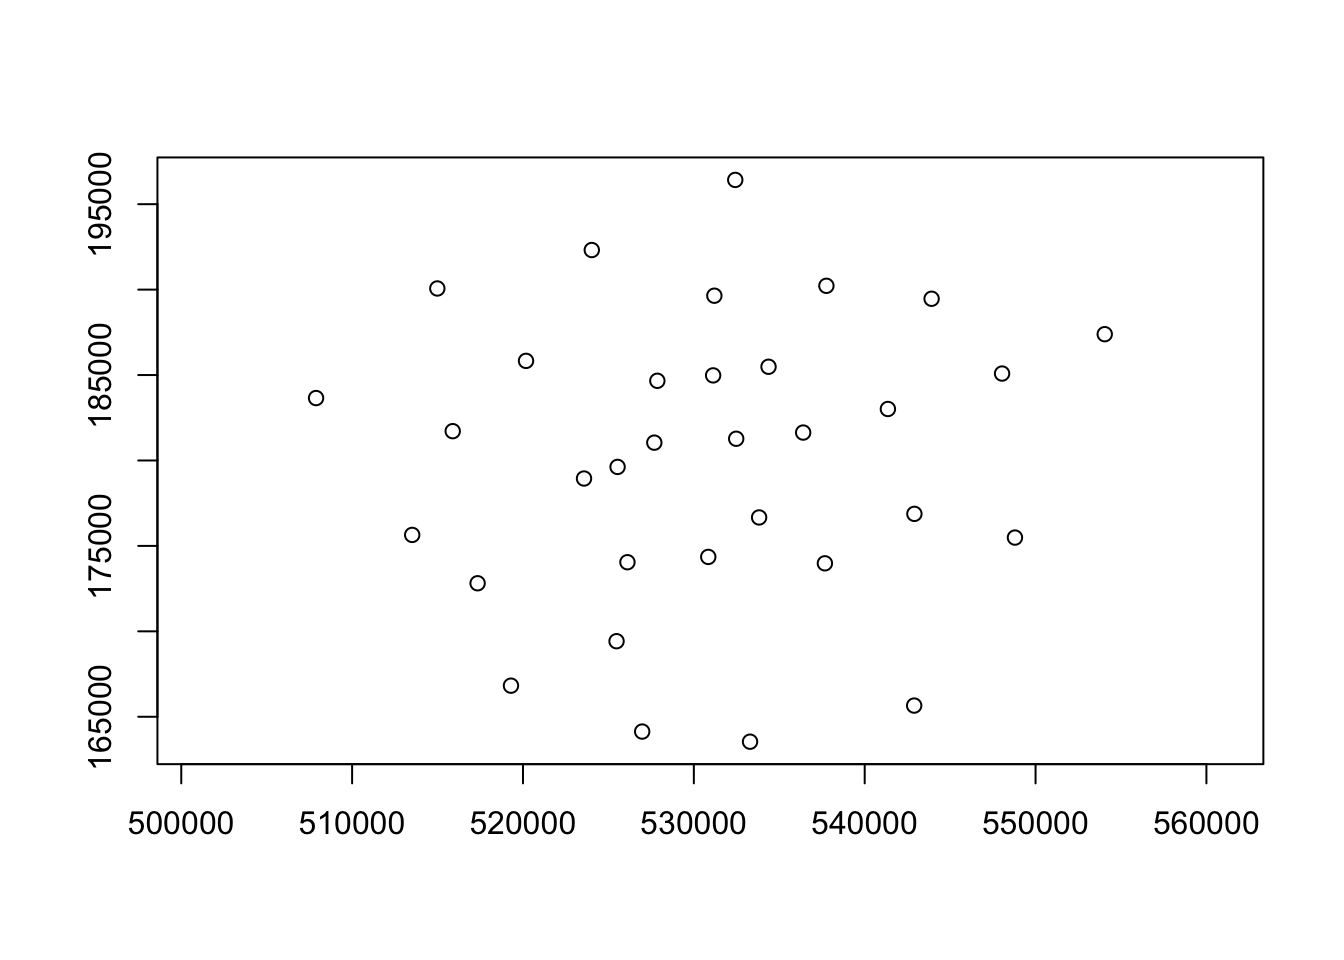
\includegraphics{bookdown-demo_files/figure-latex/unnamed-chunk-18-1.pdf}

Create a neighbours list

\begin{Shaded}
\begin{Highlighting}[]
\NormalTok{ LWard\_nb }\OtherTok{=}\NormalTok{ nsdf }\SpecialCharTok{\%\textgreater{}\%} 
  \FunctionTok{poly2nb}\NormalTok{(.,}\AttributeTok{queen=}\NormalTok{T)}
\end{Highlighting}
\end{Shaded}

Plot the neighbours list we create

\begin{Shaded}
\begin{Highlighting}[]
\FunctionTok{plot}\NormalTok{(nsdf}\SpecialCharTok{$}\NormalTok{geometry)}
\FunctionTok{plot}\NormalTok{(LWard\_nb, }\FunctionTok{st\_geometry}\NormalTok{(coordsW), }\AttributeTok{col=}\StringTok{"blue"}\NormalTok{, }\AttributeTok{add =}\NormalTok{ T)}
\end{Highlighting}
\end{Shaded}

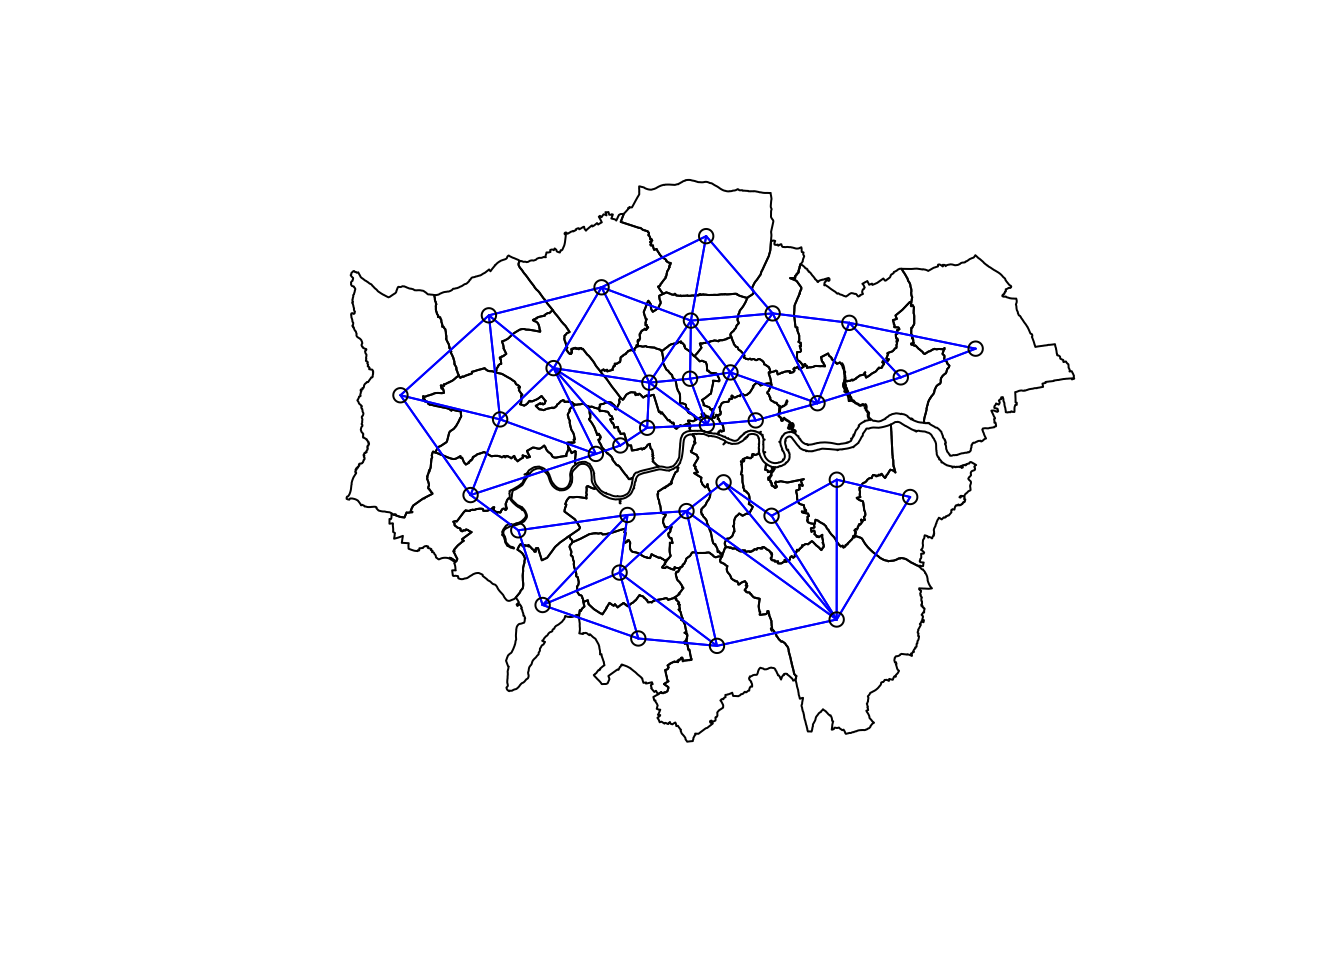
\includegraphics{bookdown-demo_files/figure-latex/unnamed-chunk-20-1.pdf}

Create a spatial weights object from these weights, which can contribute to the further analysis autocorrelation analysis (Moran's I test)

\begin{Shaded}
\begin{Highlighting}[]
\NormalTok{Lward.lw }\OtherTok{=} \FunctionTok{nb2listw}\NormalTok{(LWard\_nb, }\AttributeTok{style=}\StringTok{"C"}\NormalTok{)}
\FunctionTok{head}\NormalTok{(Lward.lw}\SpecialCharTok{$}\NormalTok{neighbours)}
\end{Highlighting}
\end{Shaded}

\begin{verbatim}
## [[1]]
## [1]  7 12 19 30 33
## 
## [[2]]
## [1] 16 25 26
## 
## [[3]]
## [1]  5  7 10 14 15
## 
## [[4]]
## [1]  6 11
## 
## [[5]]
## [1]  3  7  9 13 15 20 33
## 
## [[6]]
## [1]  4  8 11 22 23 28
\end{verbatim}

\hypertarget{calculate-the-global-morani-index}{%
\section{Calculate the Global Moran'I Index}\label{calculate-the-global-morani-index}}

Conduct the global Moran's I test to get the value.

\begin{Shaded}
\begin{Highlighting}[]
\NormalTok{ I\_LWard\_Global\_Density }\OtherTok{=}\NormalTok{ nsdf }\SpecialCharTok{\%\textgreater{}\%}
   \FunctionTok{pull}\NormalTok{(density) }\SpecialCharTok{\%\textgreater{}\%}
   \FunctionTok{as.vector}\NormalTok{()}\SpecialCharTok{\%\textgreater{}\%}
   \FunctionTok{moran.test}\NormalTok{(.,Lward.lw)}
\FunctionTok{names}\NormalTok{(I\_LWard\_Global\_Density)}
\end{Highlighting}
\end{Shaded}

\begin{verbatim}
## [1] "statistic"   "p.value"     "estimate"    "alternative" "method"     
## [6] "data.name"
\end{verbatim}

\begin{Shaded}
\begin{Highlighting}[]
\FunctionTok{head}\NormalTok{(I\_LWard\_Global\_Density)}
\end{Highlighting}
\end{Shaded}

\begin{verbatim}
## $statistic
## Moran I statistic standard deviate 
##                         0.03513093 
## 
## $p.value
## [1] 0.4859877
## 
## $estimate
## Moran I statistic       Expectation          Variance 
##      -0.028283348      -0.031250000       0.007131055 
## 
## $alternative
## [1] "greater"
## 
## $method
## [1] "Moran I test under randomisation"
## 
## $data.name
## [1] ".  \nweights: Lward.lw    \n"
\end{verbatim}

Conduct the Local Moran's I test in these two years

\begin{Shaded}
\begin{Highlighting}[]
\NormalTok{ I\_LWard\_Local\_Density }\OtherTok{=}\NormalTok{ nsdf }\SpecialCharTok{\%\textgreater{}\%}
   \FunctionTok{pull}\NormalTok{(density) }\SpecialCharTok{\%\textgreater{}\%}
   \FunctionTok{as.vector}\NormalTok{()}\SpecialCharTok{\%\textgreater{}\%}
   \FunctionTok{localmoran}\NormalTok{(., Lward.lw)}\SpecialCharTok{\%\textgreater{}\%}
   \FunctionTok{as\_tibble}\NormalTok{()}
\end{Highlighting}
\end{Shaded}

Merge the moran test result with the geometric dataset. The I value is stored in ``density\_Iz'' and the Z value is stored in ``density\_Iz''.

\begin{Shaded}
\begin{Highlighting}[]
\NormalTok{nsdf}\OtherTok{\textless{}{-}}\NormalTok{nsdf}\SpecialCharTok{\%\textgreater{}\%}
   \FunctionTok{mutate}\NormalTok{(}\AttributeTok{density\_I =} \FunctionTok{as.numeric}\NormalTok{(I\_LWard\_Local\_Density}\SpecialCharTok{$}\NormalTok{Ii))}\SpecialCharTok{\%\textgreater{}\%}
   \FunctionTok{mutate}\NormalTok{(}\AttributeTok{density\_Iz =}\FunctionTok{as.numeric}\NormalTok{(I\_LWard\_Local\_Density}\SpecialCharTok{$}\NormalTok{Z.Ii)) }
\FunctionTok{summary}\NormalTok{(nsdf}\SpecialCharTok{$}\NormalTok{density\_I)}
\FunctionTok{summary}\NormalTok{(nsdf}\SpecialCharTok{$}\NormalTok{density\_Iz)}
\end{Highlighting}
\end{Shaded}

\hypertarget{interactive-visulisation-of-the-distribution-of-the-local-moran-results}{%
\section{Interactive visulisation of the distribution of the local Moran results}\label{interactive-visulisation-of-the-distribution-of-the-local-moran-results}}

For drawing an interactive map, you should set ``view'' variables in \texttt{tmap\_mode} function. You can set break box by the minimum and maximum value of Moran.

\begin{Shaded}
\begin{Highlighting}[]
\FunctionTok{tmap\_mode}\NormalTok{(}\StringTok{"view"}\NormalTok{)}
\end{Highlighting}
\end{Shaded}

\begin{verbatim}
## tmap mode set to interactive viewing
\end{verbatim}

\begin{Shaded}
\begin{Highlighting}[]
\CommentTok{\#set the group and colour}
\FunctionTok{summary}\NormalTok{(nsdf}\SpecialCharTok{$}\NormalTok{density\_Iz)}
\end{Highlighting}
\end{Shaded}

\begin{verbatim}
##      Min.   1st Qu.    Median      Mean   3rd Qu.      Max. 
## -1.813183 -0.007425  0.133178  0.046786  0.449411  0.975067
\end{verbatim}

\begin{Shaded}
\begin{Highlighting}[]
\CommentTok{\# breaks1 = seq({-}3,1,0.5)}
\NormalTok{breaks1 }\OtherTok{=} \FunctionTok{c}\NormalTok{(}\SpecialCharTok{{-}}\DecValTok{2}\NormalTok{,}\SpecialCharTok{{-}}\DecValTok{1}\NormalTok{,}\SpecialCharTok{{-}}\FloatTok{0.1}\NormalTok{,}\SpecialCharTok{{-}}\FloatTok{0.01}\NormalTok{,}\DecValTok{0}\NormalTok{,}\FloatTok{0.01}\NormalTok{,}\FloatTok{0.1}\NormalTok{,}\FloatTok{0.45}\NormalTok{,}\DecValTok{1}\NormalTok{,}\FloatTok{1.5}\NormalTok{ ) }
\CommentTok{\# breaks2 = c({-}1000,{-}2.58,{-}1.96,{-}1.65,1.65,1.96,2.58,1000)}
\CommentTok{\# Depends on the max and min value in Moran\textquotesingle{}s I}
\NormalTok{MoranColours }\OtherTok{=} \FunctionTok{rev}\NormalTok{(}\FunctionTok{brewer.pal}\NormalTok{(}\DecValTok{8}\NormalTok{, }\StringTok{"RdGy"}\NormalTok{))}
\CommentTok{\# Plot the map}
\FunctionTok{tm\_shape}\NormalTok{(nsdf) }\SpecialCharTok{+}
  \FunctionTok{tm\_polygons}\NormalTok{(}\StringTok{"density\_Iz"}\NormalTok{,}
              \AttributeTok{style=}\StringTok{"fixed"}\NormalTok{,}
              \AttributeTok{breaks=}\NormalTok{breaks1,}
              \AttributeTok{palette=}\NormalTok{MoranColours,}
              \AttributeTok{midpoint=}\ConstantTok{NA}\NormalTok{,}
              \AttributeTok{title=}\StringTok{"Local Moran\textquotesingle{}s I,EV charge points in London"}\NormalTok{)}
\end{Highlighting}
\end{Shaded}

\hypertarget{htmlwidget-8c8d6a3296cbf651a9cf}{}

\hypertarget{gi-score}{%
\section{GI score}\label{gi-score}}

You can repeat the similar process as you can in 5.4 section to do the data preparation.

\begin{Shaded}
\begin{Highlighting}[]
\NormalTok{Gi\_LWard\_Local\_Density }\OtherTok{=}\NormalTok{ nsdf }\SpecialCharTok{\%\textgreater{}\%}
  \FunctionTok{pull}\NormalTok{(density) }\SpecialCharTok{\%\textgreater{}\%}
  \FunctionTok{as.vector}\NormalTok{()}\SpecialCharTok{\%\textgreater{}\%}
  \FunctionTok{localG}\NormalTok{(., Lward.lw)}

\CommentTok{\# To get the Min and Max value}
\FunctionTok{summary}\NormalTok{(Gi\_LWard\_Local\_Density)}
\end{Highlighting}
\end{Shaded}

\begin{verbatim}
##    Min. 1st Qu.  Median    Mean 3rd Qu.    Max. 
## -0.8861 -0.4445 -0.1112  0.1998  0.4569  2.6561
\end{verbatim}

Calculate the Gi score and transform the data type into numeric one.

\begin{Shaded}
\begin{Highlighting}[]
\NormalTok{Gi\_nsdf }\OtherTok{=}\NormalTok{ nsdf }\SpecialCharTok{\%\textgreater{}\%}
  \FunctionTok{mutate}\NormalTok{(}\AttributeTok{density\_G =} \FunctionTok{as.numeric}\NormalTok{(Gi\_LWard\_Local\_Density))}
\end{Highlighting}
\end{Shaded}

Based on the summary result of GI score to set the scale of breaks. Finally, the interactive map of Gi score distribution can be created.

\begin{Shaded}
\begin{Highlighting}[]
\NormalTok{GIColours }\OtherTok{=} \FunctionTok{rev}\NormalTok{(}\FunctionTok{brewer.pal}\NormalTok{(}\DecValTok{8}\NormalTok{, }\StringTok{"RdBu"}\NormalTok{))}

\CommentTok{\# This breaks box bases on the summary result:}
\CommentTok{\#    Min. 1st Qu.  Median    Mean 3rd Qu.    Max. }
\CommentTok{\# {-}0.8861 {-}0.4445 {-}0.1112  0.1998  0.4569  2.6561 }
\NormalTok{breaks\_GI }\OtherTok{=} \FunctionTok{c}\NormalTok{(}\SpecialCharTok{{-}}\DecValTok{2}\NormalTok{,}\SpecialCharTok{{-}}\FloatTok{1.5}\NormalTok{,}\SpecialCharTok{{-}}\DecValTok{1}\NormalTok{,}\SpecialCharTok{{-}}\FloatTok{0.4}\NormalTok{,}\SpecialCharTok{{-}}\FloatTok{0.2}\NormalTok{,}\DecValTok{0}\NormalTok{,}\FloatTok{0.2}\NormalTok{,}\FloatTok{0.5}\NormalTok{,}\DecValTok{1}\NormalTok{,}\DecValTok{2}\NormalTok{,}\FloatTok{2.5}\NormalTok{,}\DecValTok{3}\NormalTok{)}

\CommentTok{\# Now plot on an interactive map}
\FunctionTok{tmap\_mode}\NormalTok{(}\StringTok{"view"}\NormalTok{)}
\end{Highlighting}
\end{Shaded}

\begin{verbatim}
## tmap mode set to interactive viewing
\end{verbatim}

\begin{Shaded}
\begin{Highlighting}[]
\FunctionTok{tm\_shape}\NormalTok{(Gi\_nsdf) }\SpecialCharTok{+}
    \FunctionTok{tm\_polygons}\NormalTok{(}\StringTok{"density\_G"}\NormalTok{,}
        \AttributeTok{style=}\StringTok{"fixed"}\NormalTok{,}
        \AttributeTok{breaks=}\NormalTok{breaks\_GI,}
        \AttributeTok{palette=}\NormalTok{GIColours,}
        \AttributeTok{midpoint=}\ConstantTok{NA}\NormalTok{,}
        \AttributeTok{title=}\StringTok{"Gi*, EV charge points in London"}\NormalTok{)}
\end{Highlighting}
\end{Shaded}

\hypertarget{htmlwidget-848be7c37abdac5dbc3f}{}

  \bibliography{book.bib,packages.bib}

\end{document}
